


\subsection{An algorithm to discover the k-clique cover in networks~\cite{cavique2009algorithm}}


Khác với các hướng tiếp cận trước đó như [cite: 15] (dựa trên lý thuyết tập hợp) hay [cite: 16] (dựa trên cây tìm kiếm đệ quy), nghiên cứu [cite: 17] đề xuất một mô hình hai giai đoạn nhằm giải quyết bài toán bao phủ k-clique theo hướng toàn cục. Thay vì thực hiện các phép chỉnh sửa trực tiếp trên đồ thị, toàn bộ cấu trúc mạng được ánh xạ sang một biểu diễn ma trận phủ, qua đó ``làm phẳng'' độ phức tạp của bài toán đồ thị.

\subsubsection{Ý tưởng thuật toán}

Thuật toán đề xuất được chia thành hai pha độc lập nhưng liên kết chặt chẽ:
\begin{itemize}
	\item Pha 1: Tìm kiếm cụm bằng Meta-heuristic (Tabu Search). Không gian nghiệm được xây dựng thông qua các cấu trúc lân cận $N(S)$, với $S$ là tập đỉnh hiện tại. Ba toán tử chuyển trạng thái được định nghĩa.
	\begin{itemize}
		\item Thêm đỉnh: $N^+(S)={S'=S \cup \{v_i\}}$, với điều kiện vẫn bảo toàn tính chất k-clique.
		\item Xóa đỉnh: $N^-(S)={S'=S \backslash \{v_i\}}$.
		\item Hoán đổi: $N^0(S)={S'=S \cup \{v_i\} \backslash \{v_i\}}$.
	\end{itemize}
	Thông qua các toán tử này, thuật toán Tabu Search khám phá không gian nghiệm và thu thập tập các k-clique cực đại tiềm năng.
	
	\item Pha 2: Biểu diễn bài toán dưới dạng ma trận Set Covering. Sau khi hoàn tất pha tìm kiếm cụm, đồ thị ban đầu không còn được sử dụng. Thay vào đó, bài toán được chuyển sang một ma trận nhị phân $M[i,j]$ trong đó: Dòng  $i \in V$: đại diện cho các đỉnh cần được bao phủ; Cột $j \in C$: đại diện cho các cụm k-clique thu được từ pha 1; Biến quyết định $x_j \ in \{0,1\}$: xác định việc chọn cụm $j$.
	
	
\end{itemize}



















%
%Tài liệu này là bản mẫu về định dạng cho các bài báo in trên Tạp chí Khoa học và Công nghệ - Đại học Tây Bắc. Các yêu cầu cụ thể về định dạng, cấu trúc bài báo cũng được trình bày trong từng phần. 
%
%\textbf{Nếu bản thảo được soạn thảo bằng LaTex}, tác giả cần định dạng trang PDF xuất ra theo các quy định dưới đây. Bài báo phải được trình bày trên khổ A4 theo chiều dọc, với các thông số PageSetup cụ thể như sau: Top: 2 cm, Bottom: 2 cm, Left: 3,0 cm, Right: 2 cm, Header: 2,85cm, Footer: 2,85cm. Nội dung bài báo gõ bằng font chữ Times New Roman, cỡ 11, không dãn hay co cỡ chữ; chế độ dãn dòng: Single, khoảng trống dòng: before: 0, after: 0; căn lề justified. Khoảng thụt đầu dòng của đoạn văn là 0,5 cm. Tiêu đề các phần không thụt đầu dòng. Khoảng trống dòng của tiêu đề: before 6, after 6. Hình 1 mô tả thông số định dạng dãn dòng cho văn bản nội dung bài báo và thông số cho các tiêu đề.
%
%
%\setlength{\intextsep}{0pt}
%\renewcommand{\scalefigure}{0.73}
%\noindent
%\begin{figure}[h!]
%	\centering
%	\begin{subfigure}{.48\linewidth}
%		\centering
%		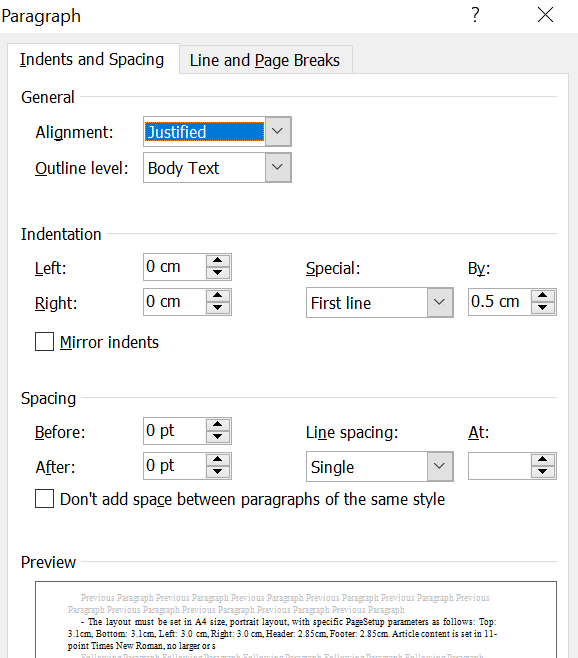
\includegraphics[scale=\scalefigure]{Pictures/pic1a.png}
%		\caption{}
%		\label{fig:format_a}
%	\end{subfigure}   
%	\begin{subfigure}{.48\linewidth}
%		\centering
%		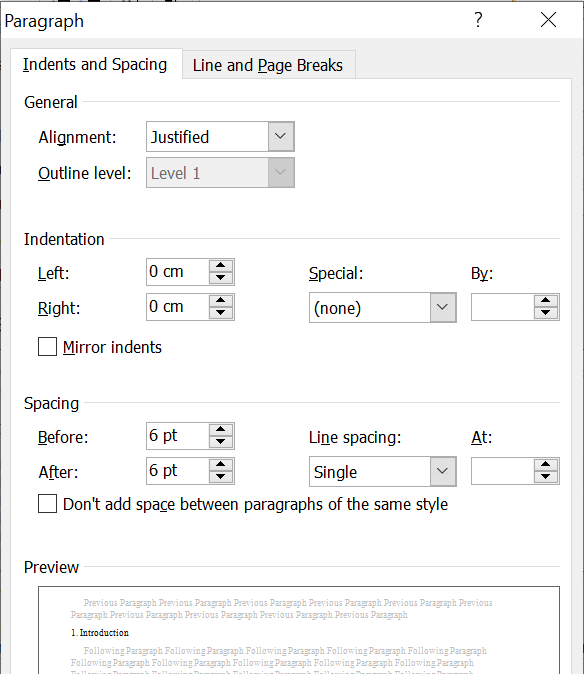
\includegraphics[scale=\scalefigure]{Pictures/pic1b.png}
%		\caption{}
%		\label{fig:format_b}
%	\end{subfigure}
%	\caption{Thông số định dạng cho (a): văn bản nội dung, (b): tiêu đề các phần}
%	\label{fig:format}
%\end{figure}
%
%Dung lượng mỗi bài báo không quá tám (08) trang, trừ những bài báo tổng quan (Review) – dung lượng từng bài dạng này do Ban biên tập xem xét cụ thể.
%
%Với bài báo soạn thảo bằng MS. Word, tác giả có thể không cần định dạng theo mẫu này. Tòa soạn sẽ dàn trang nếu bài báo được chấp nhận đăng.
%
%Bài báo cần được viết theo cấu trúc IMRAD (Introduction – Methods/Materials – Results – And Discussion. Cấu trúc IMRAD là một cấu trúc đặc thù, phổ biến trong cộng đồng khoa học quốc tế. Tiêu đề các phần chính của bài báo (Tiêu đề cấp 1) dùng chữ in đậm, cùng cỡ chữ (11 pt) với cỡ chữ của nội dung bài báo. Tiêu đề cấp 2 dùng chữ in đậm, nghiêng. Tiêu đề cấp 3 dùng chữ in nghiêng. Ví dụ định dạng tiêu đề các cấp như sau:\\
%\textbf{1. Tiêu đề cấp 1}\\
%\textbf{\textit{1.1. Tiêu đề cấp 2}}\\
%\textit{1.1.1. Tiêu đề cấp 3}\\
%\textit{1.1.2. Tiêu đề cấp 3}\\
%\textbf{\textit{1.2. Tiêu đề cấp 2}}\\
%...\\
%\textbf{\textit{2. Tiêu đề cấp 1}}
%
%\textbf{Lưu ý:} Không sử dụng chế độ đánh số tự động. Không dùng tiêu đề quá cấp 3.
%
%Nội dung phần Giới thiệu cần cung cấp những thông tin sau: vấn đề nghiên cứu đặt ra là gì, đã có những công trình nghiên cứu nào thực hiện để giải quyết vấn đề, và khoảng trống của tri thức cần được bổ sung là gì, từ đó chỉ ra mục đích nghiên cứu. Do dung lượng bài báo không quá 8 trang, nên không bố trí phần “tổng quan tài liệu” riêng.
%
%Nên cấu trúc phần Giới thiệu như sau:
%
%Trước hết, cung cấp thông tin ngắn gọn về hoàn cảnh đặt ra vấn đề cần nghiên cứu. Nếu cần, sử dụng 1-2 câu văn tóm tắt kiến thức cơ bản có liên quan trực tiếp đến vấn đề nghiên cứu. Phát biểu vấn đề nghiên cứu một cách cụ thể, súc tích. Thứ hai, thông qua việc tóm tắt các kết quả nghiên cứu liên quan đã được công bố gần nhất, chỉ ra khoảng trống về kiến thức cần bổ sung để hoàn thiện lời giải cho vấn đề nghiên cứu. Các kết quả nghiên cứu liên quan đến vấn đề nghiên cứu nhất thiết phải kèm theo trích dẫn, tham chiếu đến tài liệu tham khảo. Số lượng trích dẫn trong phần giới thiệu tối thiểu bằng số trang của bài báo, trong đó có ít nhất 5 bài báo khoa học công bố gần nhất. Nếu quá ít trích dẫn, có thể được hiểu rằng hoặc vấn đề ít quan trọng nên ít người quan tâm, hoặc tác giả không chịu tìm hiểu vấn đề đã được quan tâm giải quyết thế nào, khoảng trống kiến thức khoa học cần bổ sung là gì. Nên trích dẫn các công bố khoa học trên các tạp chí uy tín. Riêng bài báo tổng quan, cần đảm bảo có ít nhất 10 tài liệu tham khảo là các bài báo khoa học. Trong lộ trình nâng cao chất lượng Tạp chí Khoa học Đại học Tây Bắc theo chuẩn quốc tế, tác giả cần ưu tiên trích dẫn các bài báo đã đăng trên các tạp chí trong danh mục ISI, Scopus, ACI. Thông tin dùng cho trích dẫn (Metadata – siêu dữ liệu – dữ liệu mô tả) của mỗi bài báo đã đăng trên Tạp chí Khoa học Đại học Tây Bắc có thể dễ dàng download từ trang web của Tạp chí. Nếu trích dẫn từ các tạp chí trong nước, cần chỉ rõ tên đơn vị chủ quản của Tạp chí để người đọc tìm được nguồn tài liệu khi cần. 
%
%Khi trích dẫn, không nên tham chiếu đến sách giáo khoa, giáo trình, luận văn cao học. Chỉ khi nhất thiết phải sử dụng kiến thức/ công thức cơ sở trong các sách giáo trình để phát triển lý thuyết hay áp dụng cho tính toán thiết kế trong nghiên cứu thì mới trích dẫn từ các tài liệu tham khảo là sách giáo trình. 
%
%Tiếp theo, nên mô tả ngắn gọn cách thức và kết quả thu được để giải quyết vấn đề đã nêu. 
%Cuối phần Giới thiệu, nên mô tả tóm tắt nội dung các phần tiếp theo của bài báo để người đọc tiện theo dõi.
